\chapter{Triangulation}
Triangulation is a technique of computing distance of a point with respect to a known reference coordinate system, given calibration parameters, relative pose and correspondence information between imaging elements by performing optical ray-ray or optical ray-plane intersection between corresponding pixels(or plane of pixels) of imaging elements. When noise is present the optical rays may not intersect, hence typically an approximate intersection point is estimated under some assumed noise model.

\section{Current techniques for triangulation}
In this section,the current techniques used for triangulation will be briefly reviewed. This section is largely based on [4]. In this work only metric reconstruction(specifically, euclidean reconstruction) is attempted but readers interested in more detailed exposition of different types of 3D reconstructions possible given point correspondences between multiple views of the scene, can refer [3][48][49]. 
\begin{enumerate}
\item \textbf{Mid-point method}\newline
\noindent 
This method proposes to use mid-point of common perpendicular between optical rays corresponding to matching points as the intersection point.  
\\
\item \textbf{Quasi-Euclidean approach}\newline
\noindent
In this method a approximation to the correct euclidean frame is selected and mid-point method is performed in it. [4] describes it as a sub-optimal method.

\item \textbf{Linear triangulation}\newline
\noindent
Let $u_c=P*U_w$, where \textit{P} is projective transformation between a point $u_c$ in camera image plane and a point $U_w$ in world coordinate system. Here $u_c=w*(x,y,1)^T$ where 'w' is an unknown scale factor and $u_c$ is in homogenous coordinate representation. Let us denote $p_i^T$ as $i^{th}$ row of \textit{P}. This relation gives us three equations for one view:
\begin{equation}
\begin{aligned}
& w*x=p_1^T*U_w \\
& w*y=p_2^T*U_w \\
& w=p_3^T*U_w
\end{aligned}
\end{equation}

\noindent
Eliminating \textit{w}, we get two constraints on $U_w$:
\begin{equation}
\begin{aligned}
& x*(p_3^T*U_w)=p_1^T*U_w \\
& y*(p_3^T*U_w)=p_2^T*U_w
\end{aligned}
\end{equation}
\noindent
Hence using two views we get 4 equations in three unknowns which can be represented in form of system of Homogenous linear equations:
\begin{equation}
A*U=0
\end{equation}
Linear triangulation methods[50] are based on solving system of linear equations mentioned above.
\begin{enumerate}
\item \textbf{Linear-Eigen method}\newline
\noindent
Minimizes $\|AU\|$ under the constraint $\|U\|=1$. Solution is a unit eigenvector, corresponding to smallest eigenvalue of $A^T*A$. This problem may be solved using Singular-value-decomposition or Jacobi's method for finding eigenvalues of symmetric matrix.\item \textbf{Linear-LS method}\newline
\noindent
This method assumed there can be no point on plane at infinity, thereby setting w=1 in $U_w$. This constraint allows system of four linear equations for 3 unknowns whose least-squares solution can be computed using for instance Singular value decomposition method.
\end{enumerate}

\item \textbf{Iterative linear methods}\newline
\noindent
[4] points out the reason for failure of Linear method is due to lack of geometric interpretation of $\|AU\|$  and they do not minimize the optimal cost criteria proposed by them. To account for this an equivalent iterative version of methods is proposed in literature called \textit{iterative-LS} and \textit{iterative-Eigen}.  Although authors in [4] claim iterative methods to be more insensitive to projective transformations than corresponding non-iterative versions. But they also point out that non-convergence is an issue with these methods especially in the case when matching points are near epipoles, hence they suggest these methods to be used with some other supportive method which can be used in case the non-convergence is detected.

\item \textbf{Minimizing the sum-of-magnitudes of distances}\newline
\noindent
In this method, sum magnitude of Euclidean distance between observed noisy correspondence $(u_r,u_l)$ and possible candidate $(u_r^{'},u_l^{'})$ is minimized, ideal solution is the one which will exactly satisfy: 
\begin{equation}
u_r^T*F=0
\end{equation} 
where,\newline
$u_r$: position of a point in right view\newline
$u_l$: position of a point in left view\newline
F: Fundamental matrix[40]\newline
\noindent
Hence the cost function becomes:
\begin{equation}
c=d(u_r,u_r^{'})+d(u_l,u_l^{'})
\end{equation}
\noindent
where,\newline
$d(u_i,u_i^{'})$: represents the 2D euclidean distance between image points $u_i$ and $u_i^{'}$

\item \textbf{Polynomial method}\newline
\noindent
In this approach, Gaussian error model is assumed in detected features in image. It minimizes sum of squares of euclidean distances between corresponding ideal and measured points in the individual images as:
\begin{equation}
c=d(u_r,u_r^{'})^2+d(u_l,u_l^T)^2
\end{equation}
\noindent
It is proved to be optimal provided the assumed Gaussian noise-model holds. [4] argues that problem of accurate triangulation is more concerned with accurate determination of point-correspondences. This approach assumes that camera matrices(and hence fundamental matrix) is known more accurately than point-correspondences and assumption that correct matching pair will be most closer to the measured matching pair.  
\end{enumerate}

\section{Approach followed in this work}
In this work, i have actually implemented [51], Mid-point method and Linear-LS  for triangulation but it was observed that only the Linear-LS approach seems to give relatively accurate results. But it has not been analyzed in this work why other approaches do not work since our initial target was to develop a system that can perform 3D reconstruction. 

\section{Working of developed triangulation module}
For triangulation a module was developed for solving system of linear equations described in section 4.1 as Linear-LS. In used setup since it was assumed that the world coordinate system origin is at a reference plane board corner, all measurements(3D coordinates) are with respect to it. It should be noted that position of world coordinate system is not disturbed after relative extrinsic calibration of camera and projector system. Here equations described in [52] has been rephrased since these are relevant for 3D reconstruction:
Let $(u_i^c,v_i^c)$ and $(u_i^p,v_i^p)$ be the corresponding camera and projector pixels which will see $(x_i^w,y_i^w,z_i^w)$ in world. Let $A_c$,$A_p$ be the projective transformations from world-coordinate system to camera and projector coordinate system respectively. In homogeneous coordinate representation projective relations can be expressed as:\newline
\noindent
For camera:
\begin{equation}
\begin{bmatrix}
w_c*u_i^c \\
w_c*v_i^c \\
w_c
\end{bmatrix}
=\begin{bmatrix}
a_{1,1}^c & a_{1,2}^c & a_{1,3}^c & a_{1,4}^c \\
a_{2,1}^c & a_{2,2}^c & a_{2,3}^c & a_{2,4}^c \\
a_{3,1}^c & a_{3,2}^c & a_{3,3}^c & a_{3,4}^c 
\end{bmatrix}
\begin{bmatrix}
x_i^w\\
y_i^w\\
z_i^w\\
1
\end{bmatrix}
\end{equation}
\noindent
Similarly,for projector:
\begin{equation}
\begin{bmatrix}
w_c*u_i^p \\
w_c*v_i^p \\
w_p
\end{bmatrix}
=\begin{bmatrix}
a_{1,1}^p & a_{1,2}^p & a_{1,3}^p & a_{1,4}^p \\
a_{2,1}^p & a_{2,2}^p & a_{2,3}^p & a_{2,4}^p \\
a_{3,1}^p & a_{3,2}^p & a_{3,3}^p & a_{3,4}^p 
\end{bmatrix}
\begin{bmatrix}
x_i^w\\
y_i^w\\
z_i^w\\
1
\end{bmatrix}
\end{equation}
\noindent
In non-matrix form we have,\newline
\noindent
For camera,
\begin{equation}
\begin{aligned}
& w_c*u_i^c=a_{1,1}^c*x_i^w+a_{1,2}^c*y_i^w+a_{1,3}^c*z_i^w+a_{1,4}^c \\
& w_c*v_i^c=a_{2,1}^c*x_i^w+a_{2,2}^c*y_i^w+a_{2,3}^c*z_i^w+a_{2,4}^c \\
& w_c=a_{3,1}^c*x_i^w+a_{3,2}^c*y_i^w+a_{3,3}^c*z_i^w +1 \\
\end{aligned}
\end{equation}
\noindent
For projector,
\begin{equation}
\begin{aligned}
& w_p*u_i^p=a_{1,1}^p*x_i^w+a_{1,2}^p*y_i^w+a_{1,3}^p*z_i^w+a_{1,4}^p \\
& w_p*v_i^c=a_{2,1}^p*x_i^w+a_{2,2}^p*y_i^w+a_{2,3}^p*z_i^w+a_{2,4}^p \\
& w_p=a_{3,1}^p*x_i^w+a_{3,2}^p*y_i^w+a_{3,3}^p*z_i^w +1 \\
\end{aligned}
\end{equation}\newline


\noindent
Eliminating $w_p$ and $w_c$ we get,\newline
\noindent
For camera,
\begin{equation}
\begin{aligned}
& u_i^c-a_{1,4}^c=(a_{1,1}^c-u_i^c*a_{3,1}^c)*x_i^w+(a_{1,2}^c-u_i^c*a_{3,2}^c)*y_i^w+(a_{1,3}^c-u_i^c*a_{3,3}^c)*z_i^w \\
& v_i^c-a_{2,4}^c=(a_{2,1}^c-v_i^c*a_{3,1}^c)*x_i^w
+(a_{2,2}^c-v_i^c*a_{3,2}^c)*y_i^w+(a_{2,3}^c-v_i^c*a_{3,3}^c)*z_i^w \\
\end{aligned}
\end{equation}
For projector,
\begin{equation}
\begin{aligned}
& u_i^p-a_{1,4}^p=(a_{1,1}^p-u_i^p*a_{3,1}^p)*x_i^w+(a_{1,2}^p-u_i^p*a_{3,2}^p)*y_i^w+(a_{1,3}^p-u_i^p*a_{3,3}^p)*z_i^w \\
& v_i^p-a_{2,4}^p=(a_{2,1}^p-v_i^p*a_{3,1}^p)*x_i^w
+(a_{2,2}^p-v_i^p*a_{3,2}^p)*y_i^w+(a_{2,3}^p-v_i^p*a_{3,3}^p)*z_i^w \\
\end{aligned}
\end{equation}\newline
\noindent
System of equations 4.11,4.12 can be combined and written in the matrix form as:
\begin{equation}
PV=F
\end{equation}
\noindent
where,\newline
\newline
P=$\begin{bmatrix}
(a_{1,1}^c-u_i^c*a_{3,1}^c) & (a_{1,2}^c-u_i^c*a_{3,2}^c) & (a_{1,3}^c-u_i^c*a_{3,3}^c) \\ (a_{2,1}^c-v_i^c*a_{3,1}^c) & (a_{2,2}^c-v_i^c*a_{3,2}^c) & (a_{2,3}^c-v_i^c*a_{3,3}^c) \\
(a_{1,1}^p-u_i^p*a_{3,1}^p) & (a_{1,2}^p-u_i^p*a_{3,2}^p) & (a_{1,3}^p-u_i^p*a_{3,3}^p) \\ (a_{2,1}^p-v_i^p*a_{3,1}^p) & (a_{2,2}^p-v_i^p*a_{3,2}^p) & (a_{2,3}^p-v_i^p*a_{3,3}^p)
\end{bmatrix}$\newline 
\newline
\newline
\noindent
V=$\begin{bmatrix}
x_i^w\\
y_i^w\\
z_i^w
\end{bmatrix}$\newline 
\newline
\newline
\noindent
F=$\begin{bmatrix}
a_{3,4}^c*u_i^c-a_{1,4}^c\\
a_{3,4}^c*v_i^c-a_{2,4}^c\\
a_{3,4}^p*u_i^p-a_{1,4}^p\\
a_{3,4}^p*v_i^p-a_{2,4}^p
\end{bmatrix}$\newline
\noindent
\newline
Hence at each pixel $V=(P^T*P)^{-1}*P^T*F$ holds, which represents the 3D coordinate corresponding to $(u_i^c,v_i^c)$ and $ (u_i^p,v_i^p)$ in camera and projector respectively.

\section{Procedure}
Here correspondence computed from absolute phase computation step(please refer equation 3.12) is used along with the camera and projector intrinsic and extrinsic calibration parameters to compute depth. 

\section{Visualization of Point clouds}
To visualize, filter, smooth-out, down-sample and triangulate(mesh-generation from 3D data-set) the results, \textit{Point cloud library(PCL)}[53] was used. Specifically, \textit{PCL visualizer} was used for point cloud visualization. \textit{Statistical outlier detection algorithm} was used for filtering  point cloud data. \textit{Voxel-based down-sampling method} was used for reducing the number of points on rendered point cloud so as to provide relatively faster 3D rendering rate. \textit{Moving least squares(MLS)} algorithm was used for smoothing the point cloud data. \textit{Greedy triangulation algorithm} was used to generate mesh output. 3D point-clouds were also visualized in the ingeniously developed visualization tool \textit{ANUVI-v1.0.2}.
Figure~\ref{fig:3d_scans} shows snapshots of some sample 3D reconstructions using our system.


\begin{figure}[ht]
\def\tabularxcolumn#1{m{#1}}
\begin{tabularx}{\linewidth}{@{}cXX@{}}
\begin{tabular}{lr}
\subfloat[2D face image]{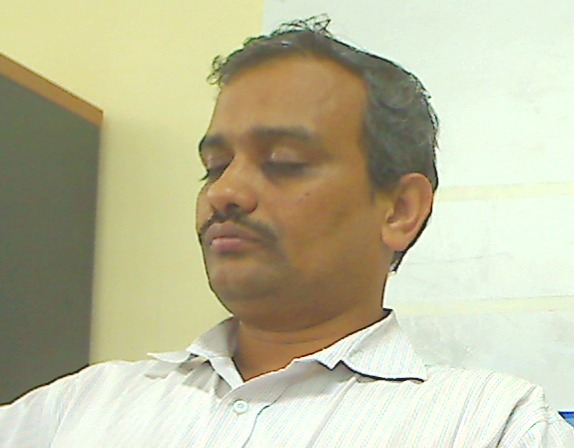
\includegraphics[width=6cm,height=5cm]{../img_source/face_2d.jpg}} 
& \hspace{1cm} \subfloat[3D reconstruction of face]{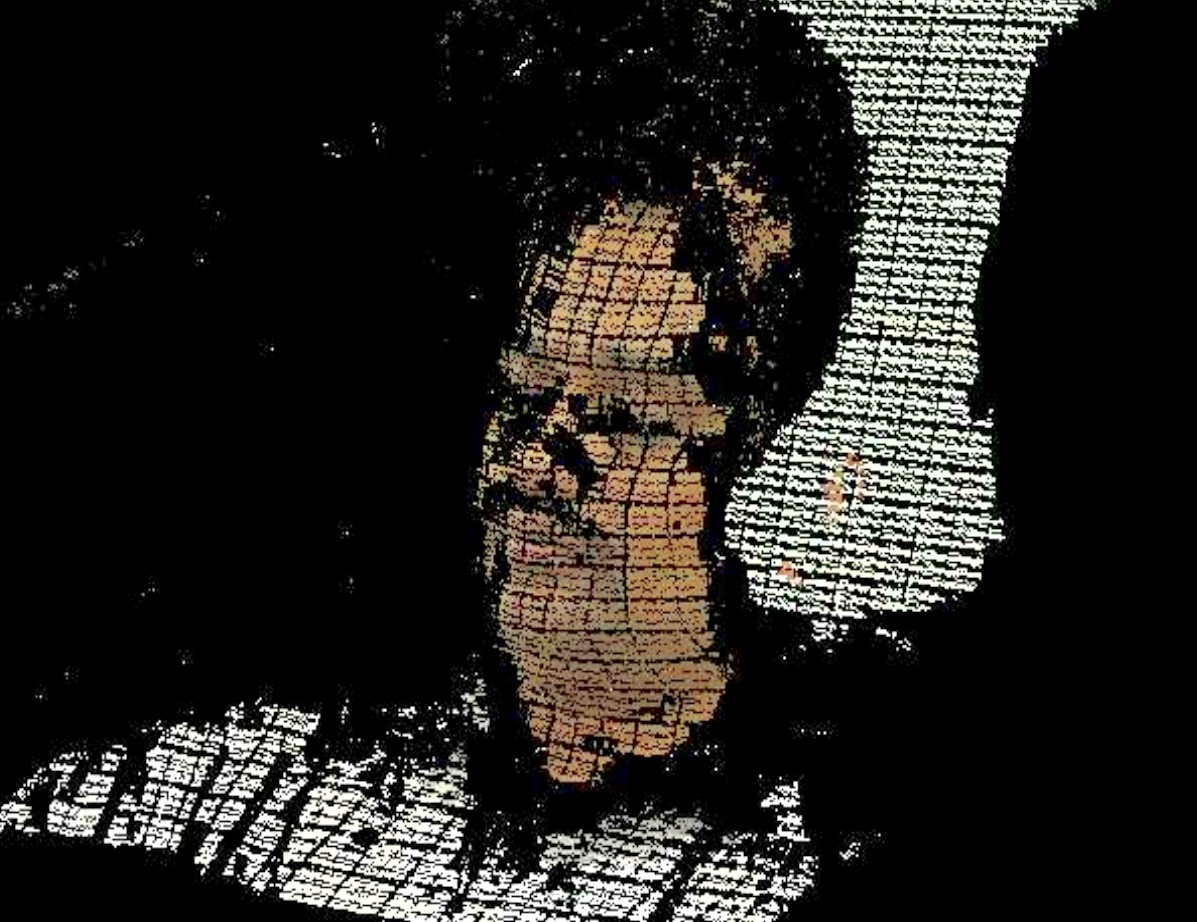
\includegraphics[width=6cm,height=5cm]{../img_source/face_3d.jpg}}\\
\subfloat[2D image of box in front of wall]{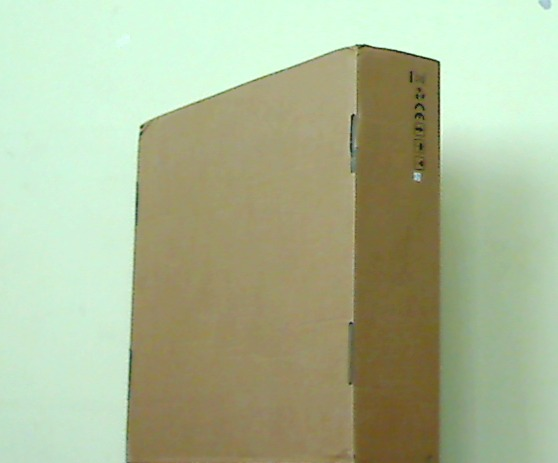
\includegraphics[width=6cm,height=5cm]{../img_source/box_wall_2d.jpg}} 
& \subfloat[3D reconstruction of box in front of wall]{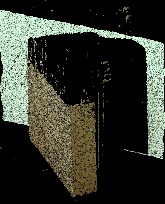
\includegraphics[width=6cm,height=5cm]{../img_source/box_wall_3d.jpg}}\\
\subfloat[2D image of a chair with background]{
\includegraphics[width=6cm,height=5cm]{../img_source/chair_2d.jpg}}
& \subfloat[3D reconstruction of chair with background]{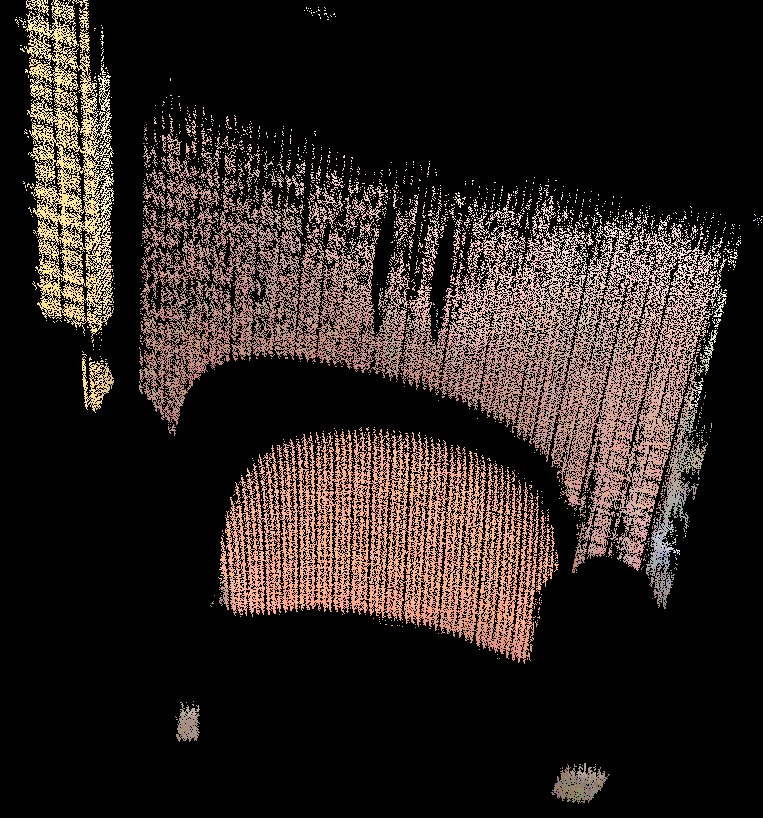
\includegraphics[width=6cm,height=5cm]{../img_source/chair_reconstruction.jpg}} \\
\subfloat[A cup]{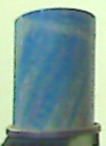
\includegraphics[width=5cm,height=5cm]{../img_source/cup_2d.jpg}}
& \subfloat[3D reconstruction of cup]{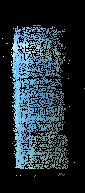
\includegraphics[width=5cm,height=5cm]{../img_source/cup_3d.jpg}}
\end{tabular}
\end{tabularx}
\caption{Some 3D reconstruction results}
\label{fig:3d_scans}
\end{figure}





\section{Discussion}
During 3D reconstruction of our reference plane(in our case it was a wall) an angle between \textit{true} reference plane(i.e., Z=0) and reconstructed plane was observed which is suspected to be because of incorrect system calibration parameters specifically extrinsic relative calibration of projector with respect to camera. This issue needs further study and experimentation to reveal the actual source of the problem.\newline
Further, evaluation of measurement accuracy(described in more detail in chapter-5) revealed average absolute relative error of $\sim$1.018\% in distance range of 1.3m to 2.5m from the developed system.   

\section{Summary}
In this chapter, a brief description of the currently used optical triangulation techniques used for metric reconstruction was presented. Further the approach used in this work for triangulation was mathematically described along with some 3D reconstruction examples to show the working of triangulation module.
